\documentclass[11pt]{article}
\usepackage[margin=1in]{geometry}
\usepackage{amsmath,amssymb,booktabs,graphicx,hyperref}
\title{Efficiency decomposition, aggregation sensitivity and reproducibility\\
in a finite-lattice overrelaxation study}
\author{ymlab analysis contributors}
\date{\today}
\begin{document}
\maketitle
\begin{abstract}
We analyse the paired overrelaxation-efficiency campaign of the Yang--Mills Mass Gap
Laboratory of Elsbernd. The per-pair ESS-per-second ratio factors exactly into a
decorrelation gain and a cost factor; in all 27 paired conditions the cost
penalty (2.8--8.4$\times$) outweighed the gain
(at most 3.11$\times$), so no ratio exceeded one (maximum 0.94).
We show that two natural aggregation rules disagree, that $\tau_{\mathrm{int}}$ is deterministic while
ESS/s is not, and report a cross-platform re-run in which hybrid chains did not reproduce.
This is a finite-lattice methodology study and makes no statement about the continuum mass gap.
\end{abstract}

\section{Setting}
The study uses the lattice and campaign of Elsbernd, \emph{Yang--Mills Mass Gap Laboratory} \url{https://github.com/Elsbernd09/yang-mills-mass-gap-lab}: SU(2) Wilson action on a
$5\times4\times4$ lattice, $\beta\in\{1.5, 2, 2.5\}$,
seeds 2026, 2027, 2028, 180 measured updates per chain, and the
schedules M, M+1OR, M+2OR, M+4OR (one Metropolis sweep followed by 0, 1, 2, 4 microcanonical overrelaxation sweeps).
The campaign and its manifests are Elsbernd's; the analysis below only post-processes
the recorded results.

\section{Symbolic models}
The following relations were derived or verified with \texttt{sympy} (\texttt{ymlab.symbolic}) and are
numerically cross-checked against the laboratory code in the test-suite.
\paragraph{Lattice coupling.} Wilson coupling for SU(N).
\begin{equation}
  \beta = \frac{2 N}{g^{2}}
\end{equation}
\paragraph{Bare coupling from beta.} bare coupling solved from the Wilson coupling relation.
\begin{equation}
  g = \frac{\sqrt{2} \sqrt{N}}{\sqrt{\beta}}
\end{equation}
\paragraph{SU(2) plaquette term.} for a unit quaternion, $\det U = a_{0}^{2} + a_{1}^{2} + a_{2}^{2} + a_{3}^{2} = 1$.
\begin{equation}
  w_{p} = 1 - a_{0}
\end{equation}
\paragraph{Effective sample size.} ESS from integrated autocorrelation time.
\begin{equation}
  N_{eff} = \frac{n_{meas}}{2 \tau}
\end{equation}
\paragraph{Efficiency ratio.} paired ESS-per-second ratio; independent of the number of measurements.
\begin{equation}
  R = \frac{t_{M} \tau_{M}}{t_{OR} \tau_{OR}}
\end{equation}
\paragraph{Break-even.} Metropolis autocorrelation time at which the efficiency ratio equals one.
\begin{equation}
  \tau_{M} = \frac{t_{OR} \tau_{OR}}{t_{M}}
\end{equation}
\paragraph{AR(1) integrated autocorrelation time.} geometric sum of autocorrelations for $|\varphi|<1$.
\begin{equation}
  \tau_{int} = \frac{\varphi + 1}{2 - 2 \varphi}
\end{equation}
\paragraph{Cosh effective mass.} the estimator ratio $[C(t-1)+C(t+1)]/2C(t)$ equals $\cosh{\left(m \right)}$, independent of $t$.
\begin{equation}
  m_{eff} = \operatorname{acosh}{\left(\cosh{\left(m \right)} \right)}
\end{equation}
\paragraph{Creutz area law.} perimeter and constant terms cancel in the Creutz ratio.
\begin{equation}
  \chi = \sigma
\end{equation}
\paragraph{O(N) mass log-slope.} logarithmic slope of the O(N) mass against $\beta$ at one loop plus the prefactor power.
\begin{equation}
  s_{O(N)} = - \frac{2 \pi}{N - 2} + \frac{1}{b \left(N - 2\right)}
\end{equation}
\paragraph{SU(N) spacing log-slope.} logarithmic slope of the lattice spacing against $\beta = 2N/g^2$ from the two-loop beta function.
\begin{equation}
  s_{SU(N)} = \frac{51}{121 b} - \frac{12 \pi^{2}}{11 N_{c}^{2}}
\end{equation}
\paragraph{One-loop coefficient (non-SUSY).} SU(N) with $n_f$ Dirac fundamentals; $b<0$ is asymptotic freedom.
\begin{equation}
  b = - \frac{11 N}{3} + \frac{2 n_{f}}{3}
\end{equation}
\paragraph{One-loop coefficient (SUSY).} SU(N) with $n_f$ chiral flavour pairs; $b<0$ is asymptotic freedom.
\begin{equation}
  b = - 3 N + n_{f}
\end{equation}

\section{Efficiency decomposition}
\begin{figure}[ht]\centering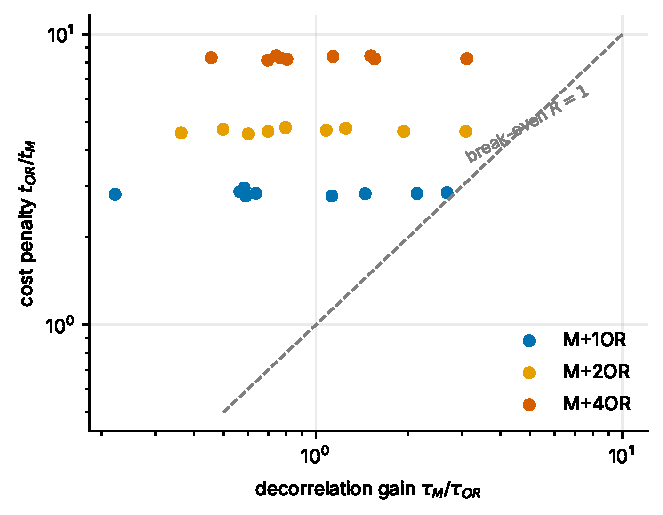
\includegraphics[width=0.62\linewidth]{gain_vs_cost}\caption{Per-pair decorrelation gain against cost penalty (log axes). Points below the dashed line would have $R>1$; none do.}\end{figure}

Across all 27 pairs the plaquette ratio lay in [0.05, 0.94];
the gain exceeded one in 12 pairs (maximum 3.11) while the cost penalty lay in
[2.8, 8.4]. For this implementation the additional sweeps were not repaid.
\begin{figure}[ht]\centering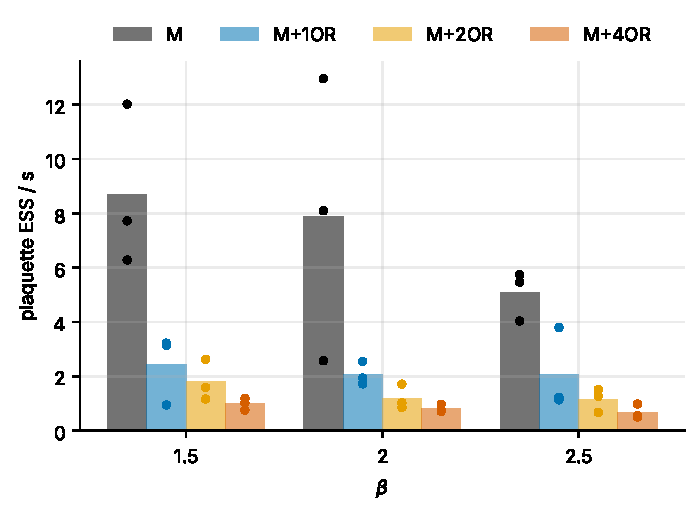
\includegraphics[width=0.62\linewidth]{ess_by_schedule}\caption{Plaquette ESS/s by schedule and $\\beta$; dots are individual seeds.}\end{figure}


\section{Aggregation sensitivity}
The mean of paired ratios and the ratio of mean ESS/s are different statistics.
\begin{table}[ht]\centering\small
\begin{tabular}{rrrrrrr}
\toprule
$\beta$ & schedule & mean gain & mean cost factor & mean of ratios & ratio of means & pair range \\
\midrule
1.5 & M+1OR & 0.93 & 0.357 & 0.333 & 0.281 & 0.08--0.51 \\
1.5 & M+2OR & 1.08 & 0.217 & 0.234 & 0.207 & 0.13--0.42 \\
1.5 & M+4OR & 1.02 & 0.122 & 0.124 & 0.114 & 0.09--0.19 \\
2 & M+1OR & 1.10 & 0.354 & 0.388 & 0.263 & 0.20--0.75 \\
2 & M+2OR & 1.32 & 0.216 & 0.284 & 0.152 & 0.08--0.67 \\
2 & M+4OR & 1.44 & 0.121 & 0.175 & 0.103 & 0.05--0.38 \\
2.5 & M+1OR & 1.30 & 0.347 & 0.454 & 0.404 & 0.20--0.94 \\
2.5 & M+2OR & 1.04 & 0.212 & 0.221 & 0.227 & 0.17--0.26 \\
2.5 & M+4OR & 1.13 & 0.119 & 0.134 & 0.133 & 0.09--0.18 \\
\bottomrule
\end{tabular}
\caption{Aggregates per $(\beta,\text{schedule})$, three seeds each.}
\end{table}
They differ by up to 86\% of the ratio of means.
\begin{figure}[ht]\centering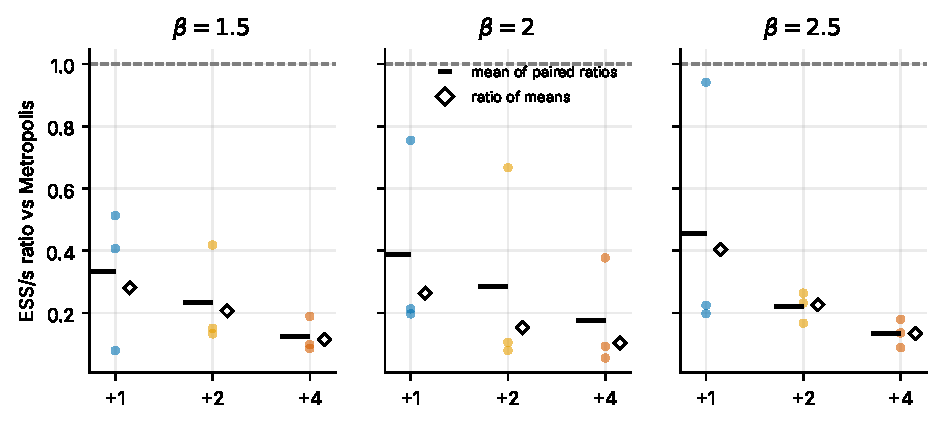
\includegraphics[width=0.95\linewidth]{aggregation_sensitivity}\caption{Per-seed ratios with the two aggregates; dashed line is break-even.}\end{figure}


\section{Determinism and reproduction}
Two published campaigns with identical configuration hash agree in $\tau_{\mathrm{int}}$ to
0.0e+00 (maximum) and in ESS/s to within 3.9\%.
\begin{figure}[ht]\centering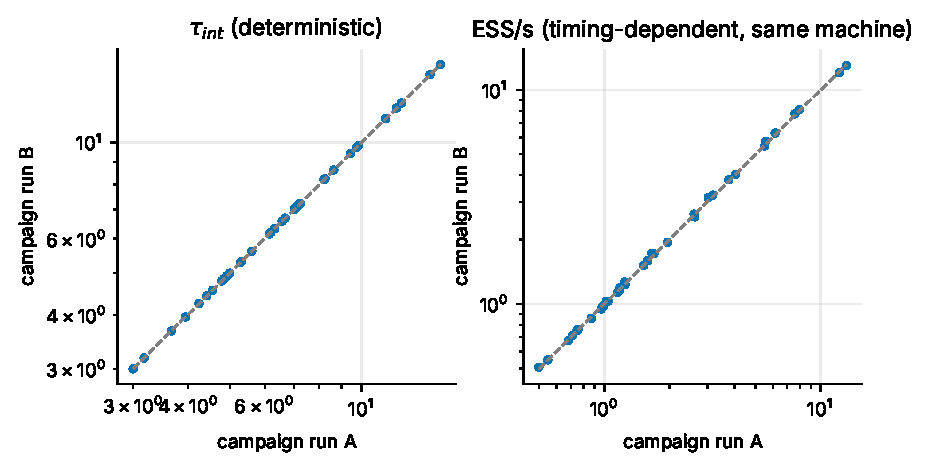
\includegraphics[width=0.85\linewidth]{determinism}\caption{Run-to-run agreement on one machine.}\end{figure}

On Linux x86\_64 (Python 3.13.18, NumPy 2.5.3) the published seed-2026 conditions were re-run; the published runs were made on Darwin arm64 (Python 3.9.6, NumPy 2.0.2). The pure-Metropolis chains reproduce the published $\tau_{int}$ to within 2.2e-13; 0 of 9 hybrid chains reproduce it exactly, with local-to-published $\tau_{int}$ ratios between 0.88 and 4.12. Median runtime here was 2.2$\times$ the published runtime. The cause of the hybrid divergence was not isolated (platform, library version, and floating-point ordering are all confounded).

\section{Asymptotic freedom: two-dimensional O(N) against four-dimensional SU(2)}
The physics tools of the OpenAI-math fork (\url{https://github.com/brentharts/openai_math_yang_mills}, commit \texttt{ba56ef3eb}) include a Wolff cluster Monte Carlo of the two-dimensional O(N) model, whose output is stored with the laboratory. The leading logarithmic slope of the mass (O(N)) or lattice spacing (SU(N)) against $\beta$ is derived with sympy; for SU(N) it is $-12\pi^2/(11N^2)$ plus a correction $51/(121\beta)$ independent of $N$.

\paragraph{O(N).} O(3): measured/predicted local slope 0.64, 0.75, 0.86 over xi = 3.4 to 11.8 (smallest L/xi 8.8); O(4): measured/predicted local slope 0.89, 0.89, 0.95 over xi = 3.0 to 14.6 (smallest L/xi 7.9). The measured slope approaches the asymptotic form from below as $\beta$ grows, which needed correlation lengths of order ten lattice spacings.
\begin{figure}[ht]\centering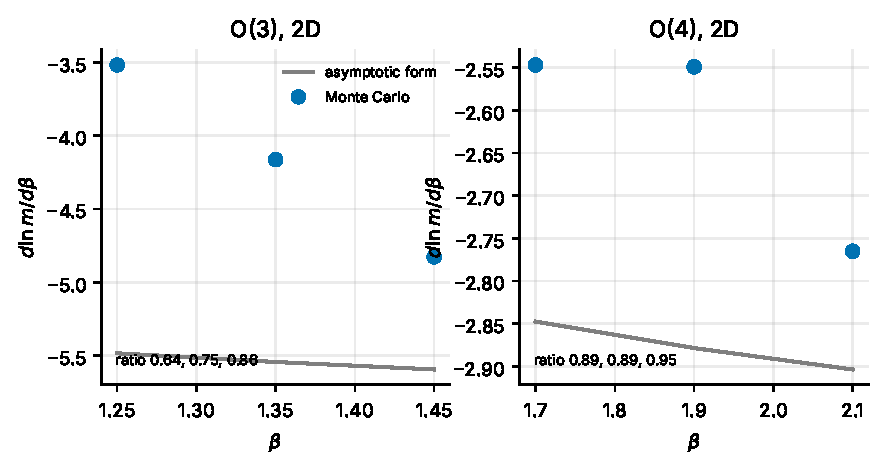
\includegraphics[width=0.85\linewidth]{on_local_slopes}\caption{Measured local slope of $\ln m$ against $\beta$ and the asymptotic form.}\end{figure}
Halving the scale takes $\Delta\beta\approx 0.12$ for O(3), 0.24 for O(4), 0.27 for SU(2) and 0.62 for SU(3) at the couplings named in the text file.

\paragraph{SU(2).} 4$^4$ lattice: measured/two-loop slope 0.74, 0.35, 0.17, 0.22, 0.20 at $\beta$ = 2.1, 2.3, 2.5, 2.7, 2.9; 6$^4$ lattice: measured/two-loop slope 0.37, 0.55, 0.22, 0.24, 0.14 at $\beta$ = 2.1, 2.3, 2.5, 2.7, 2.9.
\begin{figure}[ht]\centering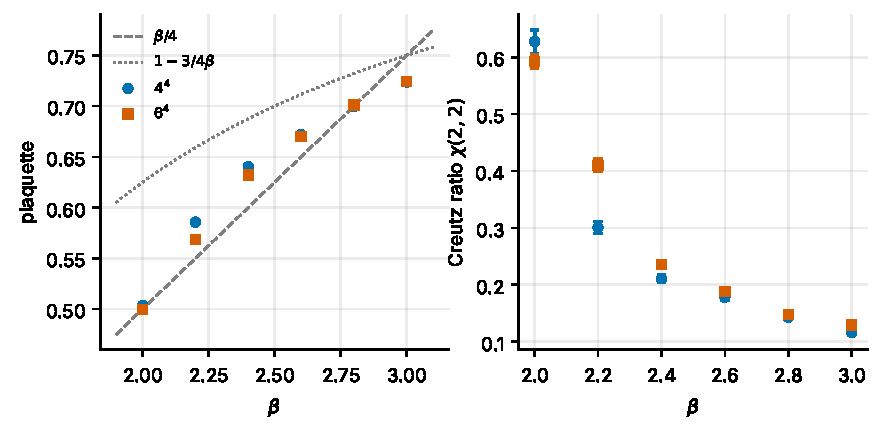
\includegraphics[width=0.85\linewidth]{su2_scan}\caption{Plaquette and Creutz ratio from the SU(2) scans; dashed and dotted lines are the leading strong- and weak-coupling terms.}\end{figure}
\begin{figure}[ht]\centering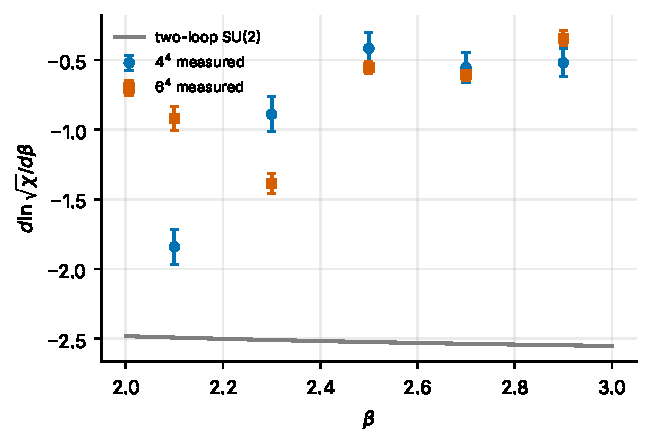
\includegraphics[width=0.6\linewidth]{su2_slopes}\caption{Measured slope of $\ln\sqrt{\chi}$ against the two-loop SU(2) slope.}\end{figure}
The SU(2) lattices are far from asymptotic scaling: the slope of ln $\sqrt{\chi}$ is 74\% of the two-loop value at best, and at most 24\% over the last three $\beta$s of every lattice (at the largest $\beta$ the ratio is 0.20 on 4$^4$ and 0.14 on 6$^4$, so the larger lattice did not move it toward one), a possible reason is strong-coupling and finite-size effects in $\chi(2,2)$ on a lattice this small, which was not tested here. The plaquette, by contrast, is already close to its weak-coupling leading term at $\beta$ of 2.8 and above (4$^4$: largest |plaquette - (1 - 3/4$\beta$)| at $\beta$ >= 2.8 is 0.032; 6$^4$: largest |plaquette - (1 - 3/4$\beta$)| at $\beta$ >= 2.8 is 0.031). The O(N) models reach 0.86 to 0.95 of the asymptotic slope at their largest $\beta$ (correlation lengths up to 15 lattice spacings); the SU(2) scans are not run at lattice sizes where a correlation length could be measured at all.

These comparisons are descriptive: the O(N) models are a toy for Yang--Mills, the SU(2) lattices are tiny with one chain per $\beta$, and nothing here concerns the continuum mass gap.

\section{One-loop cross-check with CICY}
The CICY package (\url{https://github.com/brentharts/CICY}, \texttt{pyCICY.theories.running}) computes one-loop coefficients $b_i$ from an index and uses $b_3$ in the QCD scale $\Lambda = M\exp(-2\pi/(|b_3|\alpha))$. With $d(1/\alpha)/d\ln\mu = b/2\pi$, sympy gives $b=-\tfrac{11}{3}N+\tfrac{2}{3}n_f$ (Dirac fundamentals) and $b=-3N+n_f$ (supersymmetric pairs). For $N=3$, $n_f=2n_g$ this reproduces SU(3) $b_3$: $n_g=3$: $-3$, $n_g=4$: $-1$, $n_g=5$: $+1$, the values CICY states, and $b_3=-7$ for the Standard Model; asymptotic freedom needs $n_f<3N$, at most four generations. The exponent $2\pi/(|b|\alpha)$ equals the lattice-spacing exponent $1/(2b_0g^2)$ with $b_0=-b/16\pi^2$, which is $11N/48\pi^2$ at $n_f=0$. This compares formulas with formulas; it adds no evidence about the lattice data.

\section{Limits}
Three seeds, one lattice, SU(2), plaquette emphasised; the ranking depends on the
Python/NumPy cost structure. The cross-platform divergence is observed, not explained.

\paragraph{Acknowledgement.} All simulation code, the campaign design and the recorded data are the work
of Michael Elsbernd; this document is an analysis layer on top of that work.
\end{document}
